\documentclass[12pt]{article}

\usepackage[utf8x]{inputenc} % Включаем поддержку UTF8  
\usepackage[russian]{babel}  % Включаем пакет для поддержки русского языка  
\usepackage{hyperref}        % Для гиперссылок

% Математика
\usepackage{amsmath,amsfonts,amssymb,amsthm,mathtools} % AMS
\usepackage{icomma}
\usepackage{mathrsfs}

% Прога
\usepackage{etoolbox}
\usepackage{listings}

% Цвета
\usepackage{xcolor}

% Картинки
\usepackage{graphicx}
\graphicspath{ {./images/} }

\usepackage{tikzsymbols}

% Работа с таблицами
\usepackage{array,tabularx,tabulary,booktabs} % Дополнительная работа с таблицами
\usepackage{longtable}  % Длинные таблицы
\usepackage{multirow} % Слияние строк в таблице

\newtheorem{property}{Свойство}
\newtheorem{consequence}{Следствие}[property]

\begin{document}

\thispagestyle{empty}
\begin{center}
\textbf{ПРАВИТЕЛЬСТВО РОССИЙСКОЙ ФЕДЕРАЦИИ}

\vspace{5ex}
	
\textbf{Федеральное государственное автономное образовательное учреждение \\ высшего образования \\ <<Национальный исследовательский университет \\ <<Высшая школа экономики>>}
\end{center}
\vspace{5ex}

\begin{center}
    Московский институт электроники и математики им. А.Н. Тихонова  
    
    \vspace{5ex}
    
    Департамент прикладной математики
    
    \vspace{10ex}
    \textbf{Отчёт \\ по лабораторной работе №3 \\ по курсу <<Компьютерный практикум>> \\ Вариант №7}
	\vspace{7ex}

\end{center}

\begin{center} 
\begin{tabular}{| p{0.3\linewidth}| p{0.3\linewidth}| p{0.3\linewidth}|}
 \hline	
ФИО студента & Номер группы & Дата \\  \hline
 & & \\  
Вязов Глеб \newline Дмитриевич & БПМ-231 & 10.01.2024\\  
 & & \\  \hline		
\end{tabular}
\end{center}

\begin{center}
	\vspace{3ex}
	
	\vfill
   
   \normalsize
    
	\textbf{Москва, 2023}
\end{center}

\newpage

%---------------------------------------------------------------------------------

\section*{Задание}\addcontentsline{toc}{section}{Введение}
Сделать с помощью ассемблерной вставки.
Дана строка из трех десятичных цифр. Если вторая цифра является суммой первой и третьей, то заменить ее дополнением до 9,
иначе -- поменять местами первые две цифры.

\newpage

%---------------------------------------------------------------------------------

\section*{Решение}\addcontentsline{toc}{section}{Решение}
\lstset{ %
texcl=true,%
language=C,                 % выбор языка для подсветки
basicstyle=\small\sffamily, % размер и начертание шрифта для подсветки кода
numbers=left,               % где поставить нумерацию строк (слева\справа)
numberstyle=\tiny,           % размер шрифта для номеров строк
stepnumber=1,                   % размер шага между двумя номерами строк
numbersep=5pt,                % как далеко отстоят номера строк от подсвечиваемого кода
backgroundcolor=\color{white}, % цвет фона подсветки - используем \usepackage{color}
showspaces=false,            % показывать или нет пробелы специальными отступами
showstringspaces=false,      % показывать или нет пробелы в строках
showtabs=false,             % показывать или нет табуляцию в строках
frame=single,              % рисовать рамку вокруг кода
tabsize=3,                 % размер табуляции по умолчанию равен 2 пробелам
captionpos=t,              % позиция заголовка вверху [t] или внизу [b] 
breaklines=true,           % автоматически переносить строки (да\нет)
breakatwhitespace=false, % переносить строки только если есть пробел
escapeinside={\%*}{*)},   % если нужно добавить комментарии в коде
inputencoding=utf8x,
extendedchars=\true
}

\begin{lstlisting}[label=string_code1,caption=C]
#include <stdio.h>
#include <windows.h>
#include <stdlib.h>

char* assembly(char x1, char x2, char x3) {
    char y1 = x1 - '0', y2 = x2 - '0', y3 = x3 - '0';

    __asm__ (
            ".intel_syntax noprefix \n\t"       // Меняем синтаксис AT T на синтаксис Intel

            // Сохраняем в память переменные и считаем сумму
            "mov al, %0             \n\t"       // al = x1
            "mov bl, %1             \n\t"       // bl = x2
            "mov cl, %2             \n\t"       // cl = x3
            "add al, cl             \n\t"       // al = al + cl = x1 + x3

            // Условие: сравниваем al == bl
            "cmp al, bl             \n\t"
            "je INACE               \n\t"       // Если al == cl, то переходим на метку INACE

            // Если вторая цифра НЕ равна сумме первой и третей, то меняем местами первые две цифры (al != cl)
            "mov %1, %0             \n\t"       // y2 = x1
            "mov %0, bl             \n\t"       // y1 = x2
            "jmp EXIT               \n\t"

            // Если вторая цифра равна сумме первой и третей, то y2 = 9 - x2 (al == cl)
            "INACE:                 \n\t"       // Переходим на метку INACE1
            "sub bl, 9              \n\t"       // bl = 9 - bl <= 0
            "neg bl                 \n\t"       // bl = -bl
            "mov %1, bl             \n\t"       // y2 = bl = 9 - x2

            // Выход
            "EXIT:                  \n\t"       // метка выхода
            "nop                    \n\t"
            ".att_syntax prefix;    \n\t"

            : "=r"(y1), "=r"(y2), "=r"(y3)      // выходной оператор: y1=%0, y2=%1, y3=%2
            : "0"(y1), "1"(y2), "2"(y3)         // входной оператор: x1=%3, x2=%4, x3=%5
            : "eax"                             // список разрушаемых объектов
            );

    y1 += '0', y2 += '0', y3 += '0';

    char *res = calloc(3, sizeof(char));
    res[0] = y1, res[1] = y2, res[2] = y3;

    return res;
}

char* fun(char x1, char x2, char x3) {
    char y1, y2, y3;

    if ((x2-'0') == (x1-'0') + (x3-'0')) {
        y1 = x1, y2 = (9 - (x2 - '0')) + '0', y3 = x3;
    } else {
        y1 = x2, y2 = x1, y3 = x3;
    }

    char *res = calloc(3, sizeof(char));
    res[0] = y1, res[1] = y2, res[2] = y3;

    return res;
}

int main() {
    // Меняем кодировку на UTF-8, чтобы можно было писать на русском
    SetConsoleOutputCP(CP_UTF8);
    // Ввод переменных. Дружественный интерфейс
    printf("Выполнил задание: Вязов Глеб. Группа: БПМ231\n");

    char x1, x2, x3; // байты
    char string[3];

    fgets(string, 4, stdin);
    printf("Введенная строка: %s", string);
    x1 = string[0], x2 = string[1], x3 = string[2];

    if (!(isdigit(x1) && isdigit(x2) && isdigit(x3))) {
        printf("\nНекорректный ввод!");
        return 0;
    }

    printf("\nОтвет на C: %s", fun(x1, x2, x3));
    printf("\nОтвет на ассемблере: %s", assembly(x1, x2, x3));

    return 0;
}
\end{lstlisting} 

\section*{Тестирование}\addcontentsline{toc}{section}{Тестирование}

    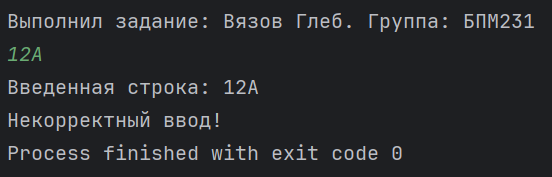
\includegraphics[width=\linewidth]{img1}
	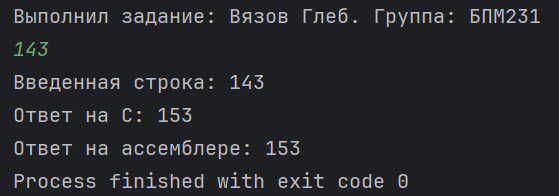
\includegraphics[width=\linewidth]{img2}
    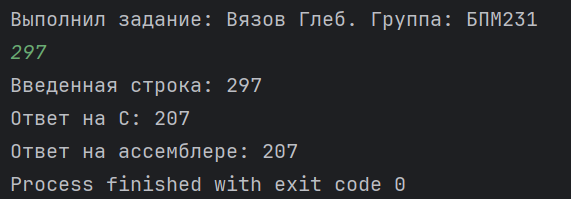
\includegraphics[width=\linewidth]{img3}
    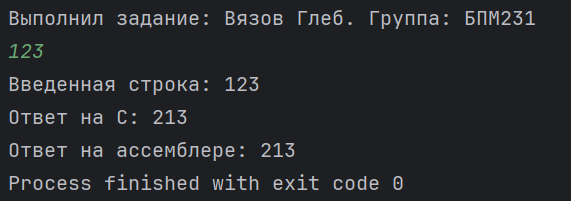
\includegraphics[width=\linewidth]{img4}

\end{document}
